\chapter{I Was Bankrupt\ldots{} Now I've Made \$3 Billion}

This chapter follows Lecture 72 in School of Hard Knocks, curated by LazyingArt LLC. We should read it not as a board lecture but as an interview whose mathematics lives inside commercial judgment: target and outcome, revenue and net, reinvestment and equity, borrowing cost and deployed return, control sets and noise sets. The lecture itself opens in compressed form, with the conclusion stated before the path is shown. Then it resets into an interview on a private jet and begins, step by step, to justify the opening boast. Our task is therefore to preserve both the numbers and the rhythm by which they are introduced.

\section{Opening Thesis: Belief Before Proof}

The lecture begins with a trailer. Sean first gives us the scale of his promise, then the realized outcome, then a warning that early wealth might have destroyed him, and only then the interview turns to its recurring question about sales. The order matters. We are first meant to feel the size of the ambition, and only afterward to ask what sort of method could possibly support it.

\paragraph{Anecdote.}
The opening pair of numbers is the anchor:
\begin{align}
G_{10} &= \$1{,}000{,}000{,}000,\\
R_{10} &\approx \$800{,}000{,}000.
\end{align}
If we form the obvious attainment ratio, we obtain
\begin{equation}
\frac{R_{10}}{G_{10}} \approx 0.8.
\end{equation}

\begin{remark}
This final ratio is editorial rather than lecture-native. Sean does not present it as a formal score. It is useful only as a compact way of seeing what the opening is doing: the original promise sounded absurd, but even partial attainment was enormous.
\end{remark}

\paragraph{Claim.}
The lecture treats long-range ambition as something that may have to be declared before evidence exists. That is the first principle. The second is that visible success is not automatically good when it arrives too early. A million dollars at twenty-two is described not as pure rescue but as a possible instrument of self-destruction.

\paragraph{Mechanism.}
So the opening tension is already double. One must believe beyond what other people think is possible, yet one must also survive one's own appetites and immaturity. This is why the teaser can move, without contradiction, from a billion-dollar promise to the claim that early money might have produced prison or death. The lecture is not praising ambition alone; it is praising ambition governed by discipline.

\section{From Broke Background to Revenue-Generating Focus}

After the teaser, the lecture resets. James introduces Sean on the private jet, and the mood changes from montage energy to long-form explanation. Sean then places himself in Connecticut, in poverty, in college athletics, in state work, and then in real estate and later multiple businesses. The biographical details are not decorative. They locate the later rules in a life that did not begin with money.

\paragraph{Anecdote.}
A key quantitative point from this early stretch is his salary as a social worker:
\begin{equation}
S_{\text{social work}} = \$58{,}000/\text{year}.
\end{equation}
That number matters because it clarifies the next transition. He does not say that he entered business because he had always worshiped money. He says instead that he wanted to provide more, give more, and no longer remain trapped by narrow income.

\paragraph{Claim.}
The first entrepreneurial filter arrives almost immediately. The real question is not whether a founder is an expert, nor whether a founder is diversified. The real question is: which line of activity actually makes money? Sean therefore insists on the paper trail. Show the P\&L. Show the net. Show EBITDA. Show that there is a real business beneath the performance.

\begin{definition}[Profitability Filter]
When several activities coexist, the first one to back heavily is the one that survives inspection by the paper trail: the P\&L, the net figure, and EBITDA. Revenue by itself does not settle the question.
\end{definition}

\begin{table}[h]
\centering
\begin{tabular}{|l|l|l|}
\hline
Measure & What it shows & Why Sean asks for it \\
\hline
Revenue & gross movement & activity can look large without real profit \\
\hline
Net & bottom-line earnings & tells us what remains after expenses \\
\hline
EBITDA & operating earnings proxy & checks the operating core of the business \\
\hline
Equity & accumulated ownership value & points to future wealth, not only current pay \\
\hline
\end{tabular}
\caption{The documentary test that separates visible activity from economic substance.}
\end{table}

\paragraph{Mechanism.}
If nine things are being done and only one of them makes money, then concentration is not a matter of taste. It is a consequence of bookkeeping. This is why the lecture rejects premature diversification. Diversity without profitable concentration is only dilution.

\subsection{Question \& Answer}

The lecture now raises a genuine local obstacle: should one follow passion, or should one follow the thing that pays?

Sean's answer is conditional, and the conditional structure is essential. A young person without dependents has room to search, to tolerate inefficiency, and to experiment. But a person with children and obligations no longer confronts the same problem. In that case, cash flow takes priority. One may need to do things one does not love in order to buy later freedom.

That is the point of the answer. The lecture refuses slogans. ``Follow your passion'' is too simple, and so is ``just chase money.'' The correct question is: what are the constraints of the present life-stage? We should therefore keep the logic conditional, not universal.

The anti-overnight-success beat belongs here as well. Sean states that he did not make a million dollars a year until his forties:
\begin{equation}
A_{\$1\text{M}} \approx 41.
\end{equation}
The point is not that everyone must wait that long. The point is that long accumulation is normal, and that the impatience of the social-media age is a bad teacher.

The lecture then pivots, quite naturally, from passion into delayed gratification. Sean says he was building businesses, feeding them, and building equity rather than maximizing current personal draw. The causal chain can be written compactly as
\begin{equation}
\text{cash flow}_t \longrightarrow \text{reinvestment}_t \longrightarrow \text{capacity}_{t+1} \longrightarrow \text{cash flow}_{t+1}.
\end{equation}
His own language is more concrete: money came in, and it went back into the business; the business was ``eating,'' and therefore it was growing. This is the bridge from life-design into the sales engine. If we are going to feed a business over time, then we need a repeatable way to generate cash. That engine is sales.

\section{The Sales Engine: Belief, Work, and Self-Image}

The lecture now returns to the question that had already been teased in the opening: why do most people struggle with sales? Sean answers the question twice in the interview, and the repetition is not accidental. It is the conceptual center of the lecture.

He begins with self-belief. Lack of self-belief leads to lack of work; lack of work weakens self-image; weak self-image undermines selling. The mechanism is given orally, but we may compress it as follows:
\begin{align}
B \downarrow &\Longrightarrow W \downarrow \Longrightarrow S \downarrow \Longrightarrow \text{sales power} \downarrow,\\
W \uparrow &\Longrightarrow S \uparrow \Longrightarrow \text{sales power} \uparrow.
\end{align}
Here \(B\) denotes self-belief, \(W\) disciplined work, and \(S\) self-image.

\paragraph{Claim.}
The sharpest line in this part of the lecture is that the best book for self-image is simply ``work.'' The claim is not mystical. One becomes harder to shake after repeated effort, repeated rejection, repeated conversation, and repeated recovery. The self-image improves because it now rests on something done, not merely on something wished for.

\begin{figure}[h]
\centering
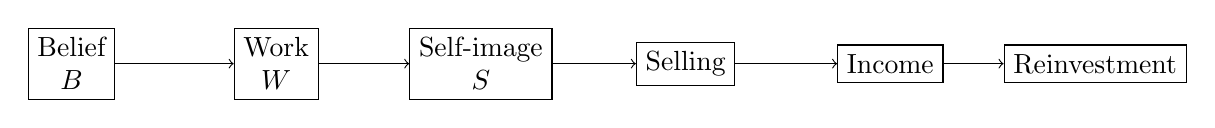
\begin{tikzpicture}[x=1cm,y=1cm]
\node[draw, align=center] (b) at (0,0) {Belief\\$B$};
\node[draw, align=center] (w) at (2.6,0) {Work\\$W$};
\node[draw, align=center] (s) at (5.2,0) {Self-image\\$S$};
\node[draw, align=center] (sell) at (7.8,0) {Selling};
\node[draw, align=center] (inc) at (10.4,0) {Income};
\node[draw, align=center] (re) at (13.0,0) {Reinvestment};

\draw[->] (b) -- (w);
\draw[->] (w) -- (s);
\draw[->] (s) -- (sell);
\draw[->] (sell) -- (inc);
\draw[->] (inc) -- (re);
\end{tikzpicture}
\caption{An editorial compression of the causal chain repeated throughout the interview.}
\end{figure}

\paragraph{Mechanism.}
The lecture then broadens the chain in three directions. First, work beats competition because most competitors simply will not work at the required level. Second, psychology matters: reading people, understanding fear, and making relationships are part of sales labor. Third, work ethic itself can become the product being sold. When pedigree and capital are absent, intensity becomes a commercial offer.

\paragraph{Anecdote.}
This is made concrete by the life-insurance story. Sean is trying to persuade a carrier to work with him. The representative gives him a long list of reasons not to do it: no experience, no capital backing, and other disadvantages. Sean's response is precise. What he has to sell is not superior balance-sheet strength. What he has to sell is work ethic. He will outwork everyone. That is the interview's turning point from motivational language to operational claim.

\begin{remark}
This is not a measured psychological model. It is a transcript-backed causal sequence. The arrows represent the structure of the lecture's explanation, not statistical coefficients.
\end{remark}

\section{Selling Yourself, Selling Truth, and Building Trust}

The lecture now narrows from sales in general to the problem of differentiation. This turn is important, and in the transcript it comes after the interruption rather than at the very beginning. The interview is resuming a second movement, not starting an unrelated topic. The question is: if products are often similar, what exactly are we selling?

\subsection{Question \& Answer}

The lecture raises the obstacle clearly. In life insurance, real estate, and waste management, the product class can look remarkably similar. The rates cluster. The service promise sounds familiar. So what is actually being sold?

Sean's answer is that the product may be near-commodity, but the operator is not. The differentiator is not metaphysical uniqueness; it is trust, reliability, responsiveness, humility, and the willingness to tell the truth when the truth is uncomfortable.

That is why the question about ``selling yourself'' is not narcissistic. The lecture does not suggest selling fantasy. It suggests making oneself a credible carrier of a product that, by itself, may not be dramatically different from the next one.

\paragraph{Claim.}
The lecture insists that confidence and humility must appear together. One should sell what one is truly good at. One should also be willing to say what one cannot do. This is not weakness. It is part of why the client can trust the strength one does claim.

\paragraph{Mechanism.}
Trust is then operationalized through small repeatable rules:
\begin{enumerate}
\item change the voicemail daily with one's own voice;
\item return calls and messages within twenty-four hours;
\item do what one says one will do;
\item obtain permission to be brutally honest;
\item then present the product, the price, and the consequences of refusal.
\end{enumerate}
This is not branding gloss. It is the interview's answer to what clients fear most. Their fear is that the seller will lie.

A very small but revealing example appears in the transcript. Once the buyer has given permission for honesty, the seller can say that the product costs \$720 a month because the buyer has had two heart attacks and cancer. The key is not the number alone. The key is that permission for truth changes the emotional structure of the conversation. Instead of dancing around reality, both parties stand inside it.

We can summarize the trust sequence in a compact way:
\begin{enumerate}
\item establish honesty as the rule;
\item obtain explicit permission for bluntness;
\item state price and consequence in the same truthful frame;
\item let reality, rather than theatrical pressure, do the selling.
\end{enumerate}

The lecture adds a second rule here: relationships deepen through acts one does not strictly owe. In Sean's language, that is where the ``currency'' of the relationship accumulates. The sale of the person is therefore not a single act of charm. It is a stock built by repeated conduct.

\section{Scaling, Delegation, and the Three-Legged Stool}

At this stage the lecture broadens from personal conduct to organizational form. The question is no longer simply how one person sells, but how a company scales without starving itself of infrastructure, patience, or leadership depth.

A key quantitative point enters here:
\begin{equation}
R_{2023} = \$752{,}000{,}000.
\end{equation}
Sean gives this number for the life-insurance business in 2023. The point of the figure is not spectacle alone. It is meant to validate the claims about distribution, infrastructure, and leadership that now follow.

\paragraph{Anecdote.}
A crucial embarrassment teaches the lesson. When a prospective buyer asks for the C-level executives, Sean realizes that he is, in practice, all of them. That is not interpreted as heroic. It is interpreted as a structural limit. One may be able to work hard enough to cover many roles for a while, but one cannot be qualified for all of them.

\paragraph{Mechanism.}
Delegation is therefore not laziness, and not merely convenience. It is role correction. A chief executive who keeps pretending to be chief financial officer and chief technology officer is not demonstrating power. He is misallocating the enterprise.

This connects directly to the mentor material. Arthur Blank's lesson is to feed the business, not starve it. Accept small margins early if the structure is right. Be patient while the business learns to breathe. Then let ``a little bit of a lot'' become enough.

\begin{definition}[Three-Legged Stool]
A business decision \(D\) is acceptable only if it is good for the client, good for the worker or agent, and not harmful to the company.
\end{definition}

In compact form,
\begin{equation}
D \text{ is admissible} \iff (D \text{ serves the client}) \land (D \text{ serves the worker}) \land \neg(D \text{ harms the firm}).
\end{equation}

\begin{table}[h]
\centering
\begin{tabular}{|l|p{8.2cm}|}
\hline
Leg & Interpretation in the lecture \\
\hline
Client & the product, service, and price must genuinely work for the buyer \\
\hline
Worker / agent & the people carrying the business must be able to win with the decision \\
\hline
Company & the decision cannot destroy long-run sustainability \\
\hline
\end{tabular}
\caption{The three-legged stool as a practical decision filter.}
\end{table}

The lecture then adds a second scaling rule, given in athletic language: do not go backwards. Sean's phrase ``never lose'' is not a full theory of finance, but it does express a compounding intuition:
\begin{equation}
r_t \ge 0 \qquad \text{for each year } t
\end{equation}
is, in his operational vocabulary, preferable to large alternating gains and losses. The principle is not that every year will be spectacular. The principle is that preserving forward motion preserves the compounding base.

Scaling also requires a social correction. Sean says companies often starve not of money but of credit. If the founder takes all the praise, then second- and third-level leadership never forms. This is why the lecture keeps shifting from ``I'' to ``we.'' Organizational scale is not only infrastructure. It is distributed dignity.

\section{Debt, Bankruptcy, and Wealth Architecture}

The lecture now moves from business design into money structure. The contrast is sharp: one way of thinking about money aims at safety through obedience, while the other treats capital as something to be deployed. Sean names the first pattern as learned behavior: get a good job, put money away, fear debt, and hope that time solves the rest.

A revealing numerical example appears in his criticism of the standard retirement script. If money is placed into a retirement account at age eighteen and cannot be touched without penalty until age \(59.5\), then the lock-up horizon is
\begin{equation}
T_{\text{lock}} = 59.5 - 18 = 41.5 \text{ years}.
\end{equation}
His objection is not that saving is irrational in every case. It is that such a structure gives someone else the use of the capital while denying the young earner the ability to deploy it into wealth-creating opportunities for more than four decades.

\paragraph{Anecdote.}
Bankruptcy then enters as a counterintuitive teacher. Sean calls it one of the best things that ever happened to him in business. The pain mattered, but the lesson mattered more: rebuild credit quickly and use restored credit as a base for new action. About a year and a half later, he reports obtaining
\begin{equation}
L_{\text{LOC}} = \$1{,}000{,}000
\end{equation}
from a local bank.

\paragraph{Claim.}
The lecture's leverage rule is simple:
\begin{equation}
r_{\text{deploy}} > r_{\text{borrow}}.
\end{equation}
That is the whole logic of why debt can be good. Borrowed money is attractive when the user can put it to work at a return above its cost.

Sean later expresses the idea in everyday numbers:
\begin{equation}
r_{\text{borrow}} \approx 3\% < 8\% \approx r_{\text{deploy}}.
\end{equation}
This is not a formal investment memorandum. It is a practical comparison. Cheap money is useful because it can be turned into more money.

\paragraph{Worked Example: Hard Money.}
The lecture's clearest financing example is the hard-money loan:
\begin{align}
L_{\text{hard}} &= \$200{,}000,\\
r_{\text{hard}} &= 12\%.
\end{align}
If we compute only the stated six-month interest cost, we obtain
\begin{equation}
\text{six-month interest} \approx 0.12 \cdot \frac{1}{2} \cdot \$200{,}000 = \$12{,}000.
\end{equation}
The transcript then adds ``10 points every six months.'' If we use the standard finance convention that one point is one percent of principal, then
\begin{equation}
\text{points over six months} \approx 0.10 \cdot \$200{,}000 = \$20{,}000.
\end{equation}
So the six-month financing cost, before repayment of principal, is approximately
\begin{equation}
\$12{,}000 + \$20{,}000 = \$32{,}000.
\end{equation}

\begin{remark}
This is a cautious standard reconstruction, not a transcript-native APR calculation. The point of the example is qualitative: once interest and points are combined, the hurdle is high. Such capital makes sense only when the project return is comfortably above the financing cost.
\end{remark}

\paragraph{Mechanism.}
The lecture's polemical edge now becomes clear. Some people see debt and see only obligation. Sean sees optionality. The same instrument that frightens the broke mindset becomes an accelerant in the hands of someone who knows what he can earn with it. Debt is therefore not good in the abstract. It is good when it is tied to competent deployment.

\section{Escaping Poverty, Surviving the Storm, and the Blueprint}

The last major movement returns from capital structure to lived entry conditions. Sean goes back to bankruptcy, broke years, transactional mentorship, and the need to escape a local script that tells people they will remain where they began. He then carries the same logic into crisis and ends by compressing the whole lecture into advice for a twenty-year-old who wants visible wealth.

\paragraph{Claim.}
The lecture rejects the slogan that the poor are fated to remain poor. Its counterclaim is not motivational vapor. It is procedural. Get around people who make money. Ask questions. Learn to sell. Teach others to sell. Build distribution. Sales is the equalizer because entry cost is relatively low and scale arrives when recruiting and teaching begin.

\paragraph{Mechanism.}
We may summarize the poverty-escape sequence as follows:
\begin{enumerate}
\item begin with low capital and weak network;
\item enter sales, where effort can substitute for inherited assets;
\item work until self-image improves;
\item use sales income to fund business building;
\item recruit and teach others;
\item convert individual effort into distribution.
\end{enumerate}

The lecture is equally precise about crisis. Whether the problem is a temporary restraining order or a burned incinerator, the first move is to identify what can actually be acted upon.

\begin{definition}[Control Partition]
In a crisis, divide the present mess into two sets: the things that can be acted upon now and the things that cannot.
\end{definition}

We may write this as
\begin{equation}
\text{Problem set} = \mathcal{C} \sqcup \mathcal{N},
\end{equation}
where \(\mathcal{C}\) is the control set and \(\mathcal{N}\) is the noise set. The corresponding action rule is
\begin{equation}
\text{Act on } \mathcal{C}, \qquad \text{do not spend the day living in } \mathcal{N}.
\end{equation}

This is how the lecture handles pressure. The court order arrives, and the next question is: what happens if it is violated? The incinerator burns down, and the next questions are: where can the trash go, who owns the landfills, who knows whom, what can be negotiated, what can be triangulated? The environment may be hostile, but the action begins only after the controllable slice has been separated out.

\subsection{Question \& Answer}

The interview ends with a deliberately visible question: how does someone come to own a private jet?

Sean's answer is corrective. Buying is not the main problem. Maintenance is. The carrying cost is the real teacher:
\begin{equation}
C_{\text{jet,idle}} \gtrsim \$150{,}000/\text{month}.
\end{equation}
That number matters because it converts the jet from a symbol into an economic object. Wealth is not the ability to buy a trophy once. It is the ability to support an expensive structure over time.

The blueprint that follows is therefore more serious than the image that prompts it. Find a good attorney and a good accountant early. Seek capital from local banks and from people who can see value in you. Ask better questions. Learn to communicate across classes and roles. Become willing to be uncomfortable. Stay humble, teachable, and non-egotistical. And then, once again, the lecture returns to the same answer it has been giving all along: become great at sales.

\section{Summary}

The lecture begins with a billion-dollar promise and ends with a beginner's blueprint. Between those two points it builds a coherent commercial philosophy. We first learn to distrust appearances and ask for paper. We then learn that sales is not merely persuasion but a chain linking belief, work, self-image, trust, and distribution. Next we learn that wealth is built less by early extraction than by feeding the business, sharing credit, and making decisions that satisfy the client, the worker, and the firm at once. Finally, we learn that debt, crisis, and discomfort are not to be romanticized, but neither are they to be feared in the abstract. They are to be handled with structure, with judgment, and with the stubborn discipline of doing the next controllable thing.